\section*{Resultados Parciais}
Uma das formas de inspecionar o aprendizado de uma rede neural artificial é pela análise dos gráficos \texttt{Acurácia x Época} e \texttt{Perda x Época}, como das figuras \ref{fig:conv_train} e \ref{fig:pretrained_train}. A análise destes dados permite saber o quanto a rede aprende por época de treinamento. Ela é importante para sabermos por quantas épocas um modelo suporta ser treinado. Sendo assim, uma forma útil -- mas não única -- de mitigação de \emph{overfiting}\footnote{Excesso ou falta de treinamento de uma rede neural articial.}.

Pela figura \ref{fig:conv_train} é visto que o \emph{overfiting} começa na oitava época de treinamento. A partir daí, a curva de perda do conjunto de validação começa a divergir da curva de perda do conjunto de treinamento.

\pagebreak
\begin{figure}[h!]
  \centering
  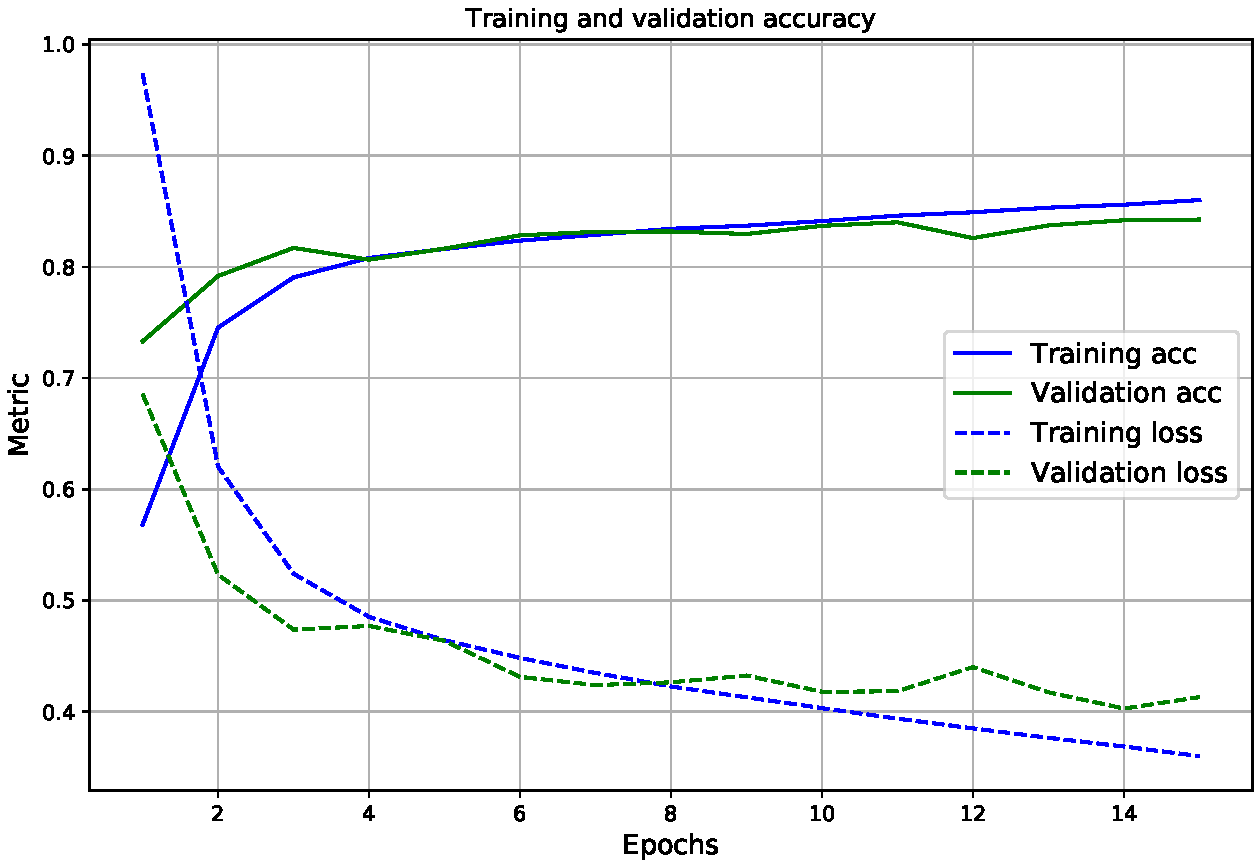
\includegraphics[width=.79\textwidth]{figures/conv_train.pdf}
  \caption{Gráfico da acurácia e perda dos subconjuntos de treino e validação em cada época de treinamento do Modelo 1.}
  \label{fig:conv_train}
\end{figure}

\begin{figure}[h!]
  \centering
  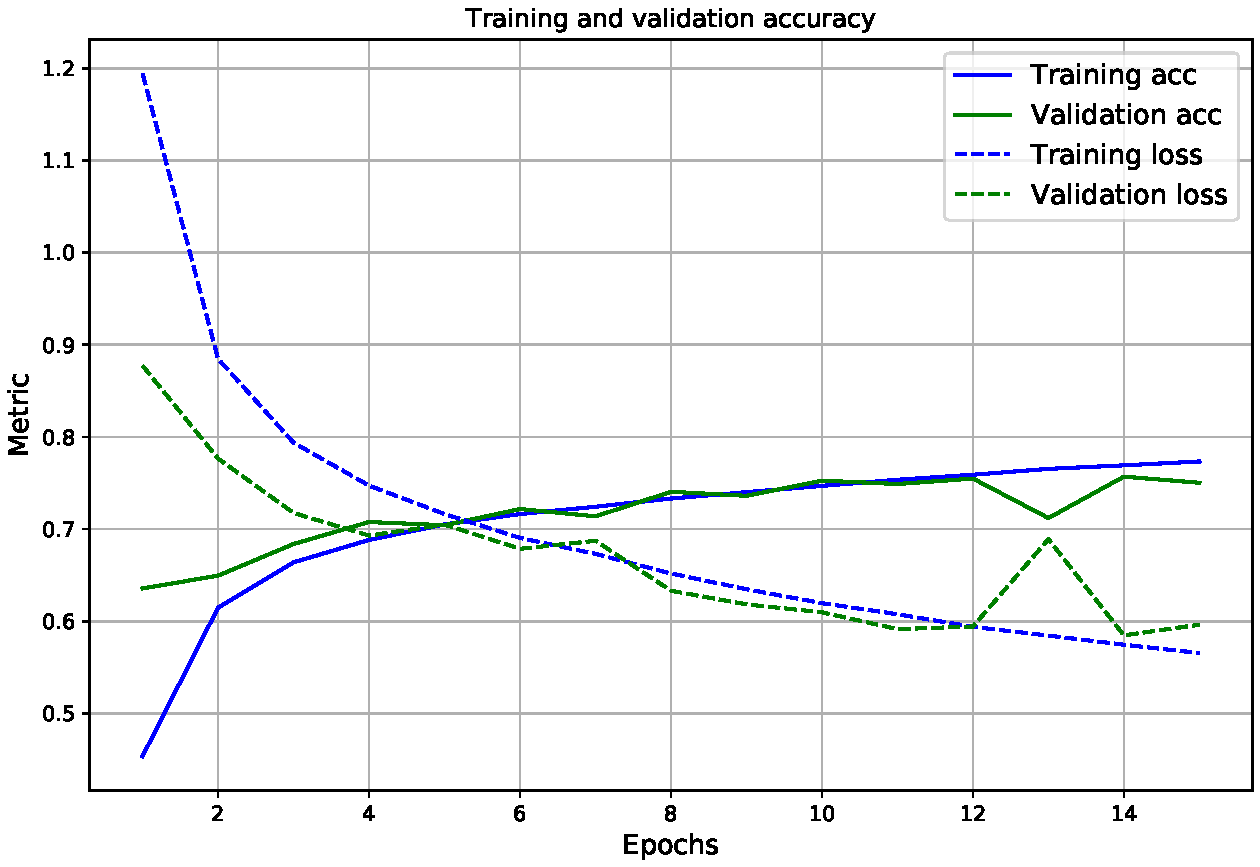
\includegraphics[width=.79\textwidth]{figures/pretrained_train.pdf}
  \caption{Gráfico da acurácia e perda dos subconjuntos de treino e validação em cada época de treinamento do Modelo 2.}
  \label{fig:pretrained_train}
\end{figure}
\pagebreak

Já na figura \ref{fig:pretrained_train} é visto que o \emph{overfiting} começa na décima segunda época de treinamento. No entanto, a acurácia final desta rede é menor que da primeira, mesmo com mais épocas de treinamento.